\documentclass[aspectratio=169]{beamer}

\usetheme{Madrid}
\usecolortheme{default}
\setbeamertemplate{navigation symbols}{}
\setbeamertemplate{footline}[frame number]

\usepackage{amsmath}
\usepackage{amssymb}
\usepackage{bm}
\usepackage{booktabs}
\usepackage{graphicx}
\usepackage{tikz}
\usetikzlibrary{arrows.meta,positioning,shapes.geometric,fit,calc}

\title{Shared-Latent Multi-Fidelity ROM for CFD-to-Experiment Transfer}
\subtitle{Methodology Draft}
\author{Project methodology presentation}
\date{\today}

\newcommand{\zs}{z_{\mathrm{s}}}
\newcommand{\zpriv}{z_f^{p}}
\newcommand{\xlf}{x^{\mathrm{LF}}}
\newcommand{\xhf}{x^{\mathrm{HF}}}
\newcommand{\mulat}{(\mu,\eta)}
\newcommand{\thetamat}{\Theta(\zs,\mu,\eta)}

\begin{document}

\begin{frame}
  \titlepage
\end{frame}

\begin{frame}{Problem Setting}
\begin{columns}[T]
\column{0.52\textwidth}
\begin{block}{Final application}
\begin{itemize}
\item Low fidelity: CFD aerosol trajectories
\item High fidelity: experiments
\item Both are high-dimensional and time-dependent
\item A paired LF-HF subset is assumed available
\end{itemize}
\end{block}

\begin{block}{Main difficulty}
\begin{itemize}
\item CFD and experiments are not separated only by noise or resolution
\item We expect nonlinear observation bias and mild evolution mismatch
\item HF data are scarce, so the surrogate must use LF efficiently
\end{itemize}
\end{block}

\column{0.48\textwidth}
\includegraphics[width=\textwidth,height=0.67\textheight,keepaspectratio]{../artifacts/notebook_cfd_like_grids/01_test_problem.png}
\end{columns}
\end{frame}

\begin{frame}{Why Not Only a Two-Step Model?}
\small
\begin{columns}[T]
\column{0.48\textwidth}
\begin{block}{Classical two-step baseline}
\[
(\mu,\eta) \mapsto \widehat x^{\mathrm{LF}}(t)
\]
\[
\widehat x^{\mathrm{HF}}(t) = G(\widehat x^{\mathrm{LF}}(t),\mu,\eta)
\]
\begin{itemize}
\item LF is mainly an intermediate predictor
\item HF stage learns a correction map
\item Simple and strong as a baseline
\end{itemize}
\end{block}

\column{0.48\textwidth}
\begin{block}{Proposed shared-latent view}
\begin{itemize}
\item LF should help learn the reduced dynamical backbone itself
\item HF should calibrate what CFD misses
\item Shared latent dynamics are the main scientific object
\end{itemize}
\[
\text{LF/HF} \rightarrow \text{shared latent core} \rightarrow \text{latent dynamics}
\]
\end{block}
\end{columns}

\vspace{0.4em}
\begin{alertblock}{Key difference}
Two-step correction uses LF as an input to a transfer map. The shared-latent strategy uses LF to reduce the sample complexity of the latent dynamical model.
\end{alertblock}
\end{frame}

\begin{frame}{Scientific Backbone}
\centering
\resizebox{\textwidth}{!}{
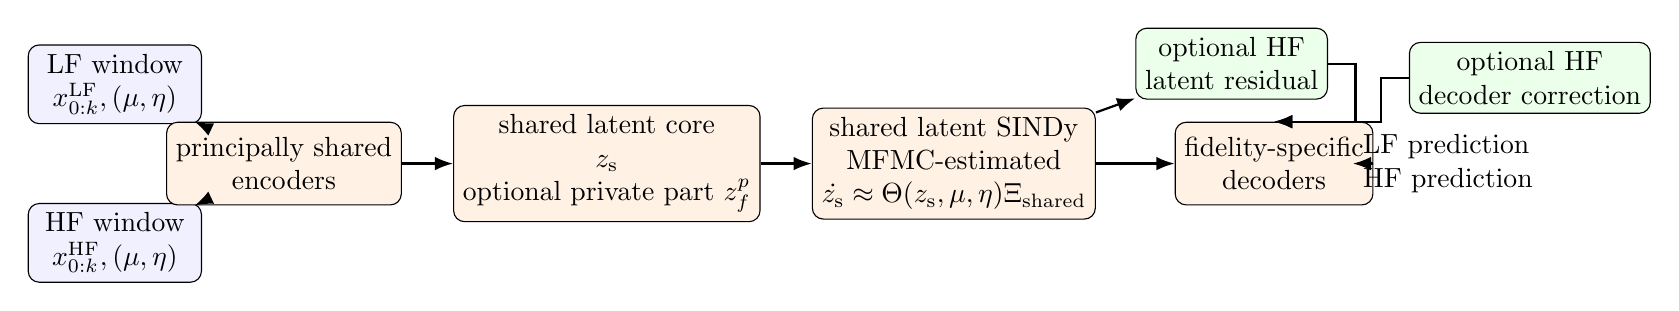
\begin{tikzpicture}[
  node distance=1.0cm and 0.65cm,
  box/.style={draw, rounded corners, align=center, minimum height=0.95cm, minimum width=2.2cm, fill=blue!6},
  block/.style={draw, rounded corners, align=center, minimum height=1.05cm, minimum width=2.5cm, fill=orange!10},
  small/.style={draw, rounded corners, align=center, minimum height=0.85cm, minimum width=1.9cm, fill=green!8},
  arr/.style={-Latex, thick}
]
\node[box] (lf) {LF window\\$\xlf_{0:k}, \mulat$};
\node[box, below=of lf] (hf) {HF window\\$\xhf_{0:k}, \mulat$};
\node[block, right=of $(lf)!0.5!(hf)$] (enc) {principally shared\\encoders};
\node[block, right=of enc] (latent) {shared latent core\\$\zs$\\optional private part $\zpriv$};
\node[block, right=of latent] (sindy) {shared latent SINDy\\MFMC-estimated\\$\dot \zs \approx \thetamat \Xi_{\mathrm{shared}}$};
\node[small, above right=0.1cm and 0.5cm of sindy] (corrdyn) {optional HF\\latent residual};
\node[block, right=1.0cm of sindy] (dec) {fidelity-specific\\decoders};
\node[small, above right=0.1cm and 0.45cm of dec] (corrdec) {optional HF\\decoder correction};

\draw[arr] (lf) -- (enc);
\draw[arr] (hf) -- (enc);
\draw[arr] (enc) -- (latent);
\draw[arr] (latent) -- (sindy);
\draw[arr] (sindy) -- (dec);
\draw[arr] (sindy) -- (corrdyn);
\draw[arr] (corrdyn.east) -- ++(0.35,0) |- (dec.north);
\draw[arr] (dec) -- ++(1.0,0) node[right, align=left] {LF prediction\\HF prediction};
\draw[arr] (corrdec.west) -- ++(-0.35,0) |- (dec.north);
\end{tikzpicture}
}

\vspace{0.4em}
\small
\begin{itemize}
\item Shared core captures common aerosol dynamics
\item Optional private/correction terms absorb CFD-to-experiment discrepancy
\item Parameter and initial-condition information enter both encoding and latent dynamics
\end{itemize}
\end{frame}

\begin{frame}{Latent Representation}
\begin{columns}[T]
\column{0.56\textwidth}
\[
E_f\!\left(x^{(f)}_{0:k}, \mu, \eta\right)
\mapsto
(\zs, z_f^p)
\]
\[
\hat x^{(f)} = D_f(\zs, z_f^p, \mu, \eta)
\]

\begin{block}{Interpretation}
\begin{itemize}
\item $\zs$: shared latent dynamical core
\item $z_f^p$: optional fidelity-specific residual information
\item $\mu,\eta$: operating parameters and initial-condition descriptors
\end{itemize}
\end{block}

\column{0.40\textwidth}
\begin{block}{Design choices}
\begin{itemize}
\item Fully shared latent state
\item Principally shared AE
\item Shared core + private latent block
\item Parameter/IC-informed encoding
\end{itemize}
\end{block}

\begin{alertblock}{Recommended default}
Start with a shared core and keep the private block optional. This is flexible enough for CFD/experiment mismatch without giving up a common latent basis.
\end{alertblock}
\end{columns}
\end{frame}

\begin{frame}{Paired LF-HF Data and Alignment}
\begin{columns}[T]
\column{0.55\textwidth}
\begin{block}{Because pairs are assumed available}
We can align the shared latent core directly on matched operating conditions and matched times.
\end{block}

\[
\mathcal{L}_{\mathrm{align}} =
\|\zs^{\mathrm{LF}} - \zs^{\mathrm{HF}}\|^2
\]
\[
\mathcal{L}_{\mathrm{roll}} =
\sum_t \|\zs^{\mathrm{LF}}(t) - \zs^{\mathrm{HF}}(t)\|^2
\]

\begin{itemize}
\item Alignment is applied to the shared core, not necessarily to the whole latent code
\item The penalty should remain soft because discrepancy is real
\end{itemize}

\column{0.45\textwidth}
\includegraphics[width=\textwidth]{../artifacts/notebook_synthetic/13_latent_diagnostics.png}
\end{columns}
\end{frame}

\begin{frame}{MFMC-SINDy on the Shared Latent Core}
\small
\begin{block}{Shared latent dynamics model}
\[
\dot \zs \approx \thetamat \, \Xi_{\mathrm{shared}}
\]
\end{block}

\begin{columns}[T]
\column{0.52\textwidth}
\begin{block}{HF target moments}
\[
C_{XX}^{\mathrm{HF}} = \mathbb{E}[\Theta^\top \Theta], \qquad
C_{XY}^{\mathrm{HF}} = \mathbb{E}[\Theta^\top \dot \zs]
\]
\end{block}

\begin{block}{MFMC estimators}
\[
\widehat C_{XY}^{\mathrm{MF}}
=
\widehat C_{XY}^{\mathrm{LF}}
+
A_{XY}\!\left(
\widehat C_{XY}^{\mathrm{HF}}
-
\widehat C_{XY}^{\mathrm{LF,p}}
\right)
\]
\[
\widehat C_{XX}^{\mathrm{MF}}
=
\widehat C_{XX}^{\mathrm{LF}}
+
A_{XX}\!\left(
\widehat C_{XX}^{\mathrm{HF}}
-
\widehat C_{XX}^{\mathrm{LF,p}}
\right)
\]
\end{block}

\column{0.44\textwidth}
\begin{block}{Why this is natural}
\begin{itemize}
\item SINDy is nonlinear in $\zs$ but linear in $\Xi_{\mathrm{shared}}$
\item LF gives low-variance moment estimates
\item Paired HF corrects LF bias
\item HF data are spent on bias correction, not on learning everything from scratch
\end{itemize}
\end{block}

\[
\Xi_{\mathrm{shared}}
=
\arg\min_{\Xi}
\|\widehat C_{XX}^{\mathrm{MF}} \Xi - \widehat C_{XY}^{\mathrm{MF}}\|_2^2
+ \beta \|\Xi\|_2^2
\]
\end{columns}
\end{frame}

\begin{frame}{Optional HF Corrections}
\begin{columns}[T]
\column{0.50\textwidth}
\begin{block}{If mismatch is mostly observational}
\[
\hat x^{\mathrm{HF}}
=
D_{\mathrm{HF}}(\zs, z_{\mathrm{HF}}^p, \mu, \eta)
+
r_{\mathrm{HF}}(\zs,\mu,\eta)
\]
\end{block}

\begin{block}{If mismatch enters the evolution}
\[
\dot \zs^{\mathrm{HF}}
\approx
\thetamat \, \Xi_{\mathrm{shared}}
+
\delta_{\mathrm{HF}}(\zs,\mu,\eta)
\]
\end{block}

\column{0.46\textwidth}
\begin{block}{Ablation order}
\begin{enumerate}
\item Shared core only
\item Shared core + HF decoder correction
\item Shared core + HF latent residual
\item Neural ODE refinement only if needed
\end{enumerate}
\end{block}

\begin{alertblock}{Reason}
The first paper should isolate how far the shared MFMC-SINDy backbone already goes before adding a stronger HF-only corrector.
\end{alertblock}
\end{columns}
\end{frame}

\begin{frame}{Staged Training Pipeline}
\begin{enumerate}
\item Train the principally shared autoencoder on LF/HF trajectories with parameter conditioning.
\item Use paired data to align the shared latent core and compute latent rollout mismatch.
\item Encode trajectories and estimate latent derivatives.
\item Build the SINDy library on the shared core.
\item Fit the shared operator with MFMC-style moment estimators.
\item Fit an optional HF correction only if the shared core is insufficient.
\item Run ablations and compare against the two-step baseline.
\end{enumerate}

\vspace{0.6em}
\begin{block}{Why staged training}
\begin{itemize}
\item It matches the mathematical role of MFMC in latent linear regression
\item It is more stable than full Neural ODE training from the start
\item It keeps the scientific decomposition interpretable
\end{itemize}
\end{block}
\end{frame}

\begin{frame}{Benchmark Illustrations}
\begin{columns}[T]
\column{0.51\textwidth}
\includegraphics[width=\textwidth,height=0.62\textheight,keepaspectratio]{../artifacts/notebook_cfd_like_grids/12_fidelity_gap.png}

\column{0.47\textwidth}
\small
\begin{block}{What the plots should show}
\begin{itemize}
\item The LF-HF gap is structured, not random noise
\item A useful model must capture both common evolution and fidelity discrepancy
\item Evaluation must include cross-fidelity gap metrics, not only per-fidelity reconstruction
\end{itemize}
\end{block}

\vspace{0.5em}
\begin{block}{Core metrics}
\begin{itemize}
\item reconstruction error
\item paired latent alignment error
\item latent SINDy residual
\item rollout error
\item fidelity-gap error
\end{itemize}
\end{block}
\end{columns}
\end{frame}

\begin{frame}{Comparison with the Two-Step Baseline}
\small
\begin{tabular}{p{0.31\textwidth}p{0.30\textwidth}p{0.31\textwidth}}
\toprule
Aspect & Two-step LF$\rightarrow$HF correction & Shared-latent MFMC-SINDy \\
\midrule
Role of LF & Intermediate prediction to be corrected & Data source for latent manifold and latent dynamics \\
Use of paired data & Mostly for learning correction map & For latent alignment and MFMC bias correction \\
Common physics & Implicit & Explicit shared latent backbone \\
HF scarcity benefit & Mostly on correction stage & On shared dynamical operator estimation \\
Interpretability & Limited & Shared core plus explicit residual decomposition \\
Training complexity & Lower & Higher, but more structured \\
\bottomrule
\end{tabular}

\vspace{0.8em}
\begin{alertblock}{Required baseline}
The two-step model remains mandatory in experiments because it is simpler, strong, and may win if CFD and experiments are too different dynamically.
\end{alertblock}
\end{frame}

\begin{frame}{Development Priorities}
\small
\begin{block}{Immediate engineering tasks}
\begin{itemize}
\item define the paired-data contract and conditioning variables
\item choose shared core only vs shared core + private latent block
\item implement latent derivative estimation and SINDy library construction
\item implement MFMC moment estimators and sparse latent solve
\item add a minimal shared-latent example and a minimal two-step baseline
\end{itemize}
\end{block}

\begin{block}{Validation tasks}
\begin{itemize}
\item dataset and pairing tests
\item SINDy library and derivative tests
\item MFMC regression unit tests
\item end-to-end pipeline smoke test
\item example-level regression checks
\end{itemize}
\end{block}
\end{frame}

\begin{frame}{Takeaway}
\begin{itemize}
\item The chosen methodology is a paired shared-latent multi-fidelity ROM with MFMC-SINDy at the latent level.
\item LF CFD trajectories are used to learn the dominant latent backbone, not only a pre-correction surrogate.
\item HF experiments calibrate what CFD misses through paired alignment and optional HF residual correction.
\item Neural ODE refinement remains possible, but it is not the first model to build.
\end{itemize}

\vspace{0.8em}
\centering
\Large
Shared latent backbone first, HF correction second, Neural ODE later if needed.
\end{frame}

\end{document}
